\documentclass{scrartcl}

\usepackage[hidelinks]{hyperref}
\usepackage[none]{hyphenat}
\usepackage{setspace}
\usepackage{graphicx}
\usepackage{wrapfig}
\graphicspath{ {images/} }
\doublespace

%Please include a clear, concise, and descriptive title
\title{An Introduction to the Sega Master System}

%Please do not change the subtitle
\subtitle{COMP130 - Game Platform History Essay}

%Please put your student ID in the author field
\author{AR185160}

\begin{document}

\maketitle




<<<<<<< HEAD
\abstract {\textbf{Abstract} \par This paper will discuss the Sega Master System game platform and will be focusing primarily on how the technical innovations that were released with the Master System paved the way for today’s technology. From the console hardware to the peripherals, this paper will evaluate which technologies that came with the console proved successful and which led to the failure of the console.}

%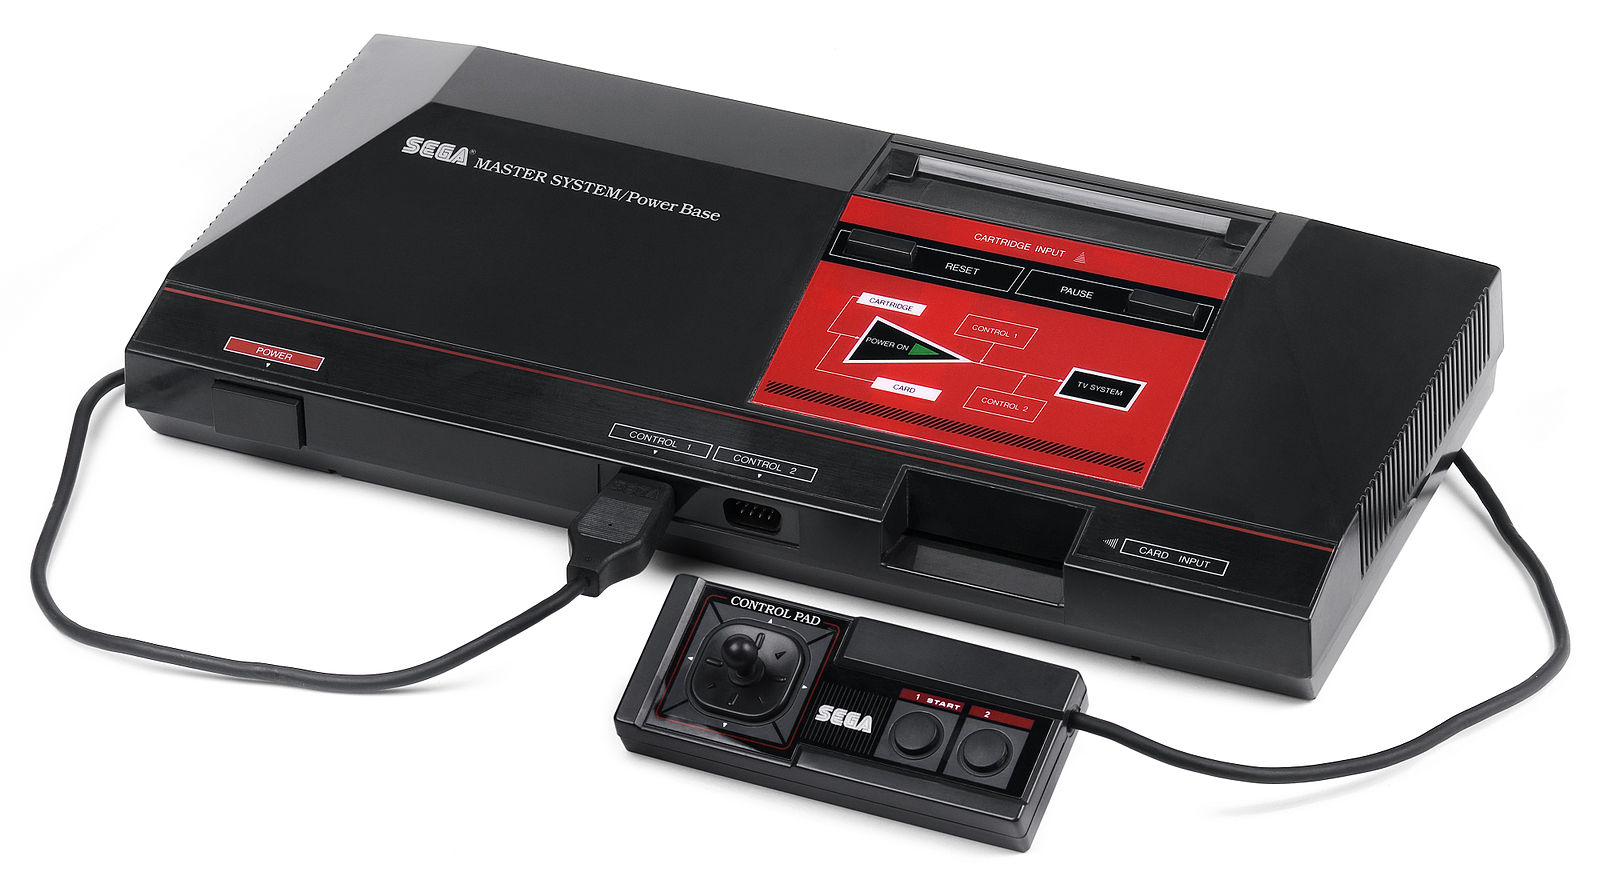
\includegraphics[scale=0.3]{Sega-Master-System.jpg}

\section{A brief overview of the Sega Master System}

The Sega Master System (also known as SMS) is a game console which was released in the late 80’s. The SMS was the second iteration of the console as it was originally released in japan in 1985 as the Sega Mark III \cite{Weiss2009}, it was later redesigned and released in North America in 1986 then again in Europe in 1987. The reason for the re-design was to appeal to the western audience by making the console look more futuristic\cite{parkin}. In 1989 Sega released the Sega Master System II, which again was completely redesigned to be a low-cost cut down version of the original.
=======
\abstract {\textbf{Abstract} \par This paper will discuss the Sega Master System game platform and will be focusing primarily on how the technical innovations that were released with the Master System paved the way for todays technology. From the console hardware to the peripherals, this paper will evaluate which technologies that came with the console proved successful and which led to the failure of the console.}

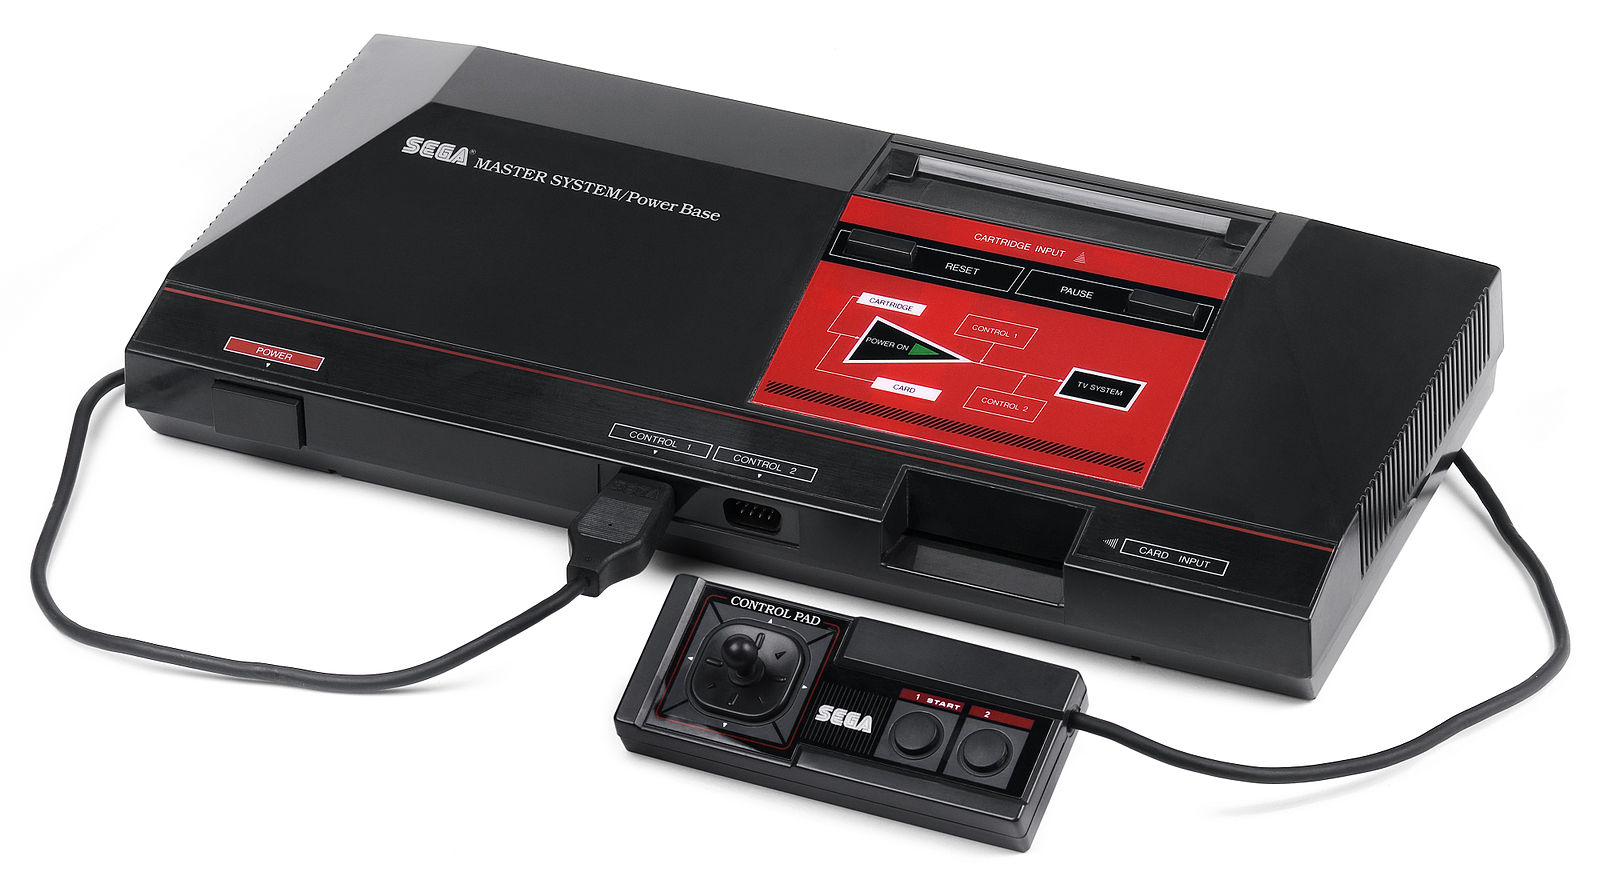
\includegraphics[scale=0.3]{Sega-Master-System.jpg}

\section{A breif overview of the Sega Master System}

The Sega Master System (also known as SMS) is a game console which was released in the late 80’s. The SMS was the second iteration of the console as it was originally released in japan in 1985 as the Sega Mark III \cite{Weiss2009}, it was later redesgined and released in North America in 1986 then again in Europe in 1987. The reason for the re-design was to appeal to the western audiance by making the console look more futuristic\cite{parkin}. In 1989 Sega released the Sega Master System II, which again was completely redesigned to be a low-cost cutdown version of the original.
>>>>>>> origin/master

The Master System is often seen as a failure because it was dwarfed by the sales of the NES, however it was still a very popular console in regions such as Europe and Brazil. For example in 1994 the Master System had the largest active console user-base in Europe, with 6.25Million active consoles.\cite{russell} And it has had a steady stream of buyers in Brazil and is still, to this day fairly popular over there.


<<<<<<< HEAD
The console was designed to rival the Nintendo Entertainment System (NES), However the SMS did not sell well in comparison, especially in America and Japan.\cite{Orland}, so this will be focusing on what technology was disfavoured over the popular NES and what Sega could have done to improve the console, additionally what did Sega do right and how did that contribute to the technology we have today.
=======
The console was designed to rival the Nintendo Entertianment System (NES), However the SMS did not sell well in coomparison, especially in America and Japan.\cite{Orland}, so this will be focusing on what technology was disfavoured over the popular NES and what Sega could have done to improve the console, additionally what did Sega do right and how did that contribute to the technology we have today.
>>>>>>> origin/master

\section{The Technology behind the System}

\textbf{Technical advances} \par

<<<<<<< HEAD
The Sega Master System had the most impressive hardware for a console in its generation, it featured a wide range of colour capabilities as it could display up to 64 colours on the screen simultaneously compared to the NES\cite{racket}, which could only display up to 48. This was thanks to the Master Systems display processor was so advanced for its time that its successor, the Mega Drive used the same graphics and sound chips. The SMS also used a Zilog Z80 processor which was a is robust microprocessor used arcade machines meaning that the console was reliable and rarely had hardware faults.\cite{russell} 

The master system came with two different types of memory card slots, the Sega Card was a relatively small credit-card size and had only 256kb (32KB) of storage and were a lot cheaper to manufacture. However most popular game developers developed their games for the standard cartridge format which could hold up to 1048Kb (131KB) of data. \cite{Weiss2009} The Master System is fully backwards compliable with the SG-1000 titles, both the card and cartridges, as well as it's controllers. \cite{racket} This difference between the two game cartridges was unique to Sega consoles and it was a clever idea so that even if you couldn't afford the more expensive cartridges, you were still able to play the smaller cheaper games that were available on the Sega cards. The console also had an innovative feature where if no game was inserted, you could play the default game that came installed on the console, the game varies on which version of the Master System you own. This was a great feature because even if you only just have the console without any games, you were still able to use it.
=======
The Sega Master System had the most impressive hardware for a console in its generation, it featured a wide range of colour capabilities as it could display upto 64 colours on the screen simultaneously compared to the NES\cite{racket}, which could only display upto 48. This was thanks to the Master Systems display processor was so advanced for its time that it's successor, the Mega Drive used the same graphics and sound chips. The SMS also used a Zilog Z80 processor which was a is robust microprocessor used arcade machines meaning that the console was reliable and rarely had hardware faults.\cite{russell} 

The master system came with two different types of memory card slots, the Sega Card was a relatively small credit-card size and had only 256kb (32KB) of storage but were a lot cheaper to manafacture. However most popular game developers developed their games for the standard cartidge format which could hold upto 1048Kb (131KB) of data. \cite{Weiss2009} The Master System is fully backwards compiable with the SG-1000 titles, both the card and cartridges, as well as it's controllers. \cite{racket} This difference between the two game cartridges was unique to Sega consoles and it was a clever idea so that even if you coun't afford the more expensive cartridges, you were still able to play the smaller cheaper games that were avalible on the Sega cards. The console also had an innovative feature where if no game was inserted, you could play the default game that came installed on the console, the game varies on which version of the Master System you own. This was a great feature because even if you only just have the console without any games, you were still able to use it.
>>>>>>> origin/master



\textbf{The Peripherals} \par

<<<<<<< HEAD
However one of the most innovative bits of technology to come with the SMS was the Segascope 3-D glasses that was able to plug into the SMS's Sega Card slot, this allowed users to view the games in 3-D and was the first time that 3D was implemented with a degree of success in the video game industry. The glasses used a similar version of the active shutter technology in the new 3D TV's today.\cite{SegaScopeTech} This was considered the beginning to VR technology in games, as a few years later in 1995 Nintendo released its Virtual Boy. \cite{Workman} The glasses were exclusive to the SMS and therefore anyone in the late 80's who was fascinated with the concept of 3-D games would have had to buy a Master System, in order to test them out.

Another nifty peripheral that was released with the SMS was the Light Phaser, the design is almost identical to the NES's zapper, however apparently it had slightly better targeting system and a more responsive trigger. 


\textbf{The unpopular features of the Sega Master System compared to the Nintendo Entertainment System.} \par

The main reason for Nintendo’s huge success over the SMS was because Nintendo launched its Nintendo Entertainment System one year before the SMS and they had a strict non-compete licencing agreement with game developers. This meant that games which were released for the NES were not allowed to be released to any other console for two years.\cite{Weiss2009} So when the Sega Master System released one year later it was left out in the cold, and could not compete with the popularity of the games on the NES. Meaning that the SMS only had a total of around 330 games that were released, compared to the NES's roughly 500. \cite{russell}

Another very unpopular feature was that the pause button was on the console it's self, not on the controller like normal video game consoles. This meant that if you need to pause the game quickly, you have to get out of your seat and press the pause button on the console! This would be a huge inconvenience when you're in the middle of a boss battle and need a quick break. Furthermore the controllers were not as pleasant as the NES controller, they had a 4 way directional pad that was apparently not as precise as Nintendo’s design.\cite{Weiss2009}
=======
However one of the most innovative bits of technology to come with the SMS was the Segascope 3-D glasses that was able to plug into the SMS's Sega Card slot, this allowed users to view the games in 3-D and was the first time that 3D was implemented with a degree of success in the video game industry. The glasses used a similar version of the active shutter technology in the new 3D TV's today.\cite{SegaScopeTech} This was considered the beginning to VR technology in games, as a few years later in 1995 Nintendo released its Virtual Boy. \cite{Workman} The glasses were exclusive to the SMS and therefore anyone in the late 80's who was facinated with the concept of 3-D games would have had to buy a Master System, in order to test them out.

Another nifty peripheral that was released with the SMS was the Light Phaser, the design is almost identical to the NES's zapper, however aparently it had slightly better targeting system and a more responsive trigger. 


\textbf{The unpopular features of the Sega Master System compared to the Nentendo Entertainment System.} \par

The main reason for Nintendos huge success over the SMS was because Nintendo launched its Nentendo Entertainment System one year before the SMS and they had a strict non-compete licencing agreement with game developers. This meant that games which were released for the NES were not allowed to be released to any other console for two years.\cite{Weiss2009} So when the Sega Master System released one year later it was left out in the cold, and could not compete with the popularity of the games on the NES. Meaning that the SMS only had a total of around 330 games that were released, compared to the NES's roughly 500. \cite{russell}

Another very unpopular feature was that the pause button was on the console it's self, not on the controller like normal video game consoles. This meant that if you need to pause the game quickly, you have to get out of your seat and press the pause button on the console! This would be a huge inconveniance when you're in the middle of a boss battle and need a quick break. Furthermore the controllers were not as pleasant as the NES controller, they had a 4 way directional pad that was aparently not as precise as Nintendos design.\cite{Weiss2009}
>>>>>>> origin/master




\section{Conclusion}

<<<<<<< HEAD


Even though Sega did so many things right with the Master System, Segas downfall was that the software and games did not meet the standard of the hardware. So if Sega managed to organise a deal with some popular game developers to make good games for their console, the Master System might have had a chance against the Nintendo Entertainment System

The Sega Master System had an innovative design and some interesting and quite revolutionary peripherals but again was let down by the lack of good, popular games. 

From all the sources I have seen about the SMS, everyone who had owned one had very little complaints and were very proud to be an owner of the console, even the games that were released on the console seemed to be loved by the Master System community.

=======
Even though Sega did so many things right with the Master System, Segas downfall was that the software and games did not meet the standard of the hardware. So if Sega managed to organise a deal with some popular game developers to make good games for their console, the Master System might of had a chance against the Nintendo Entertainment System

The Sega Master System had an innovative design and some interesting and quite revolutionary peripherals but again was let down by the lack of good, popular games. 

From all the sources I have seen about the SMS, everyone who had owned one had very little complaints are overall were very proud to be an owner of the console, and even the games that were released on the console seemed to be loved by the Master System community. 
>>>>>>> origin/master

\bibliographystyle{ieeetr}
\bibliography{game-platform-history-references}

%\begin{wrapfigure}{}{0.4\textwidth} 
 %   \centering
  %  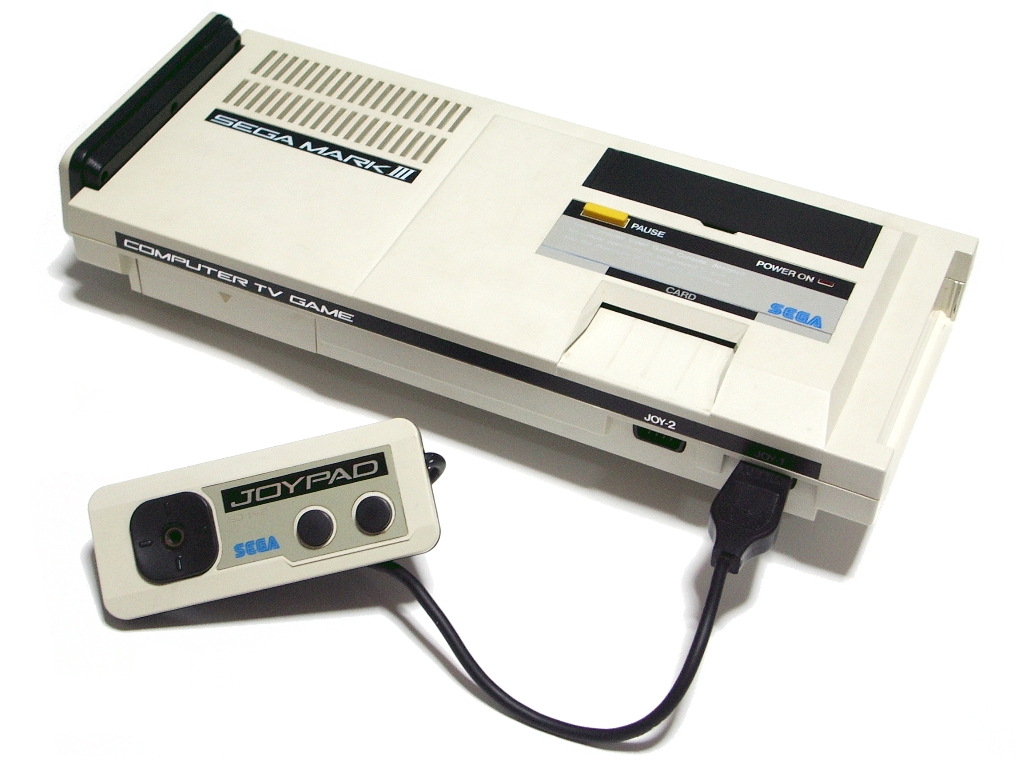
\includegraphics[scale=0.2]{Sega_Mark_III.jpg}
  %  \caption{Sega-Mark-III}
  %  \label{fig:mark_III}
%\end{wrapfigure}



\end{document}

